% =======================FLAT======STABLE=========================================================================
\begin{figure}
    \centering
    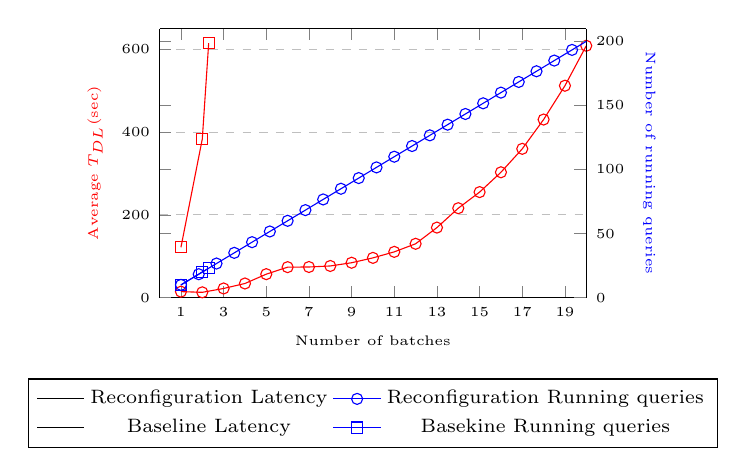
\begin{tikzpicture}
        \begin{axis}
            [
            axis y line*=left,
            ylabel style={align=center},
            xlabel style={align=center},
            xmin=0, xmax=20,
            xtick={1, 3, 5, 7, 9, 11, 13, 15, 17, 19},
            legend style={at={(0.5,-0.3)},anchor=north},
            ymajorgrids=true,
            grid style=dashed,
            axis y line*=left,
            ymin=0, ymax=650,
            xlabel={Number of batches},
            ylabel near ticks,
            width=7cm, height=5cm,
            label style={font=\tiny},
            legend columns=-2,
            legend style={font=\fontsize{7}{5}\selectfont},
            ticklabel style = {font=\tiny},
            ylabel={\textcolor{red}{Average $T_{DL}$} \\\textcolor{red}{(sec)}}
            ]
            \addplot[
                color=red,
                mark=o,
            ]
            coordinates {
                (1, 14.6719239936)(2, 13.0139209216)(3, 22.3023760384)(4, 34.3407150336)(5, 56.8850899712)(6, 73.8143830016)(7, 74.1653380352)(8, 76.6513830144)(9, 84.4626129408)(10, 96.203356032)(11, 110.7239309824)(12, 130.217201024)(13, 169.3572349952)(14, 216.13144)(15, 255.0461259776)(16, 302.9065289472)(17, 359.541545984)(18, 430.2846960128)(19, 511.9421840128)(20, 608.428076032)
            }; \label{plot:fs_10_re}
            \addplot+[
            color=red,
            mark=square,
            ]
            coordinates {(1, 121.78)(2, 383.10)(2.3, 614.80)}; \label{plot:fs_10_bas}
        \end{axis}
        \begin{axis}
            [
            axis x line=none,
            xmin=0, xmax=20,
            ymin=0, ymax=210,
            legend style={at={(0.5,-0.3)},anchor=north},
            ylabel near ticks, yticklabel pos=right,
            ylabel={\textcolor{blue}{Number of running queries}},
            width=7cm, height=5cm,
            label style={font=\tiny},
            legend columns=2,transpose legend,
            legend style={font=\fontsize{7}{5}\selectfont},
            ticklabel style = {font=\tiny},
            y label style={align=center, rotate=180}
            ]
            \addlegendimage{/pgfplots/refstyle=plot:fs_10_re}\addlegendentry{Reconfiguration Latency}
            \addlegendimage{/pgfplots/refstyle=plot:fs_10_bas}\addlegendentry{Baseline Latency}
            \addlegendentry{Reconfiguration Running queries}
            \addlegendentry{Basekine Running queries}

            \addplot[blue,smooth,mark=o,domain=1:21]{10*x};
            \addplot[blue,smooth,mark=square]
            coordinates {(1, 10)(2, 20)(2.3, 23)};
        \end{axis}

    \end{tikzpicture}
    \caption{{Average $T_{DL}$} for flat topology with stable workloads of 10 QPS}
\end{figure}

% =======================Hier======STABLE=========================================================================

\begin{figure}
    \centering
    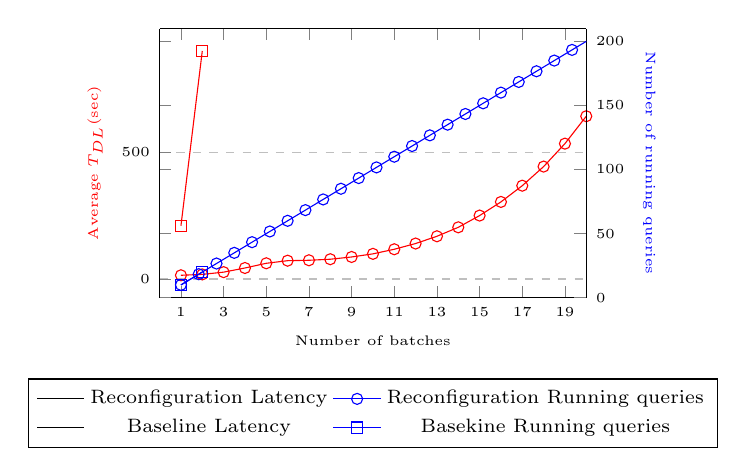
\begin{tikzpicture}
        \begin{axis}
            [
            axis y line*=left,
            ylabel style={align=center},
            xlabel style={align=center},
            xmin=0, xmax=20,
            xtick={1, 3, 5, 7, 9, 11, 13, 15, 17, 19},
            legend style={at={(0.5,-0.3)},anchor=north},
            ymajorgrids=true,
            grid style=dashed,
            axis y line*=left,
            xlabel={Number of batches},
            ylabel near ticks,
            width=7cm, height=5cm,
            label style={font=\tiny},
            legend columns=2,transpose legend,
            legend style={font=\fontsize{7}{5}\selectfont},
            ticklabel style = {font=\tiny},
            ylabel={\textcolor{red}{Average $T_{DL}$} \\\textcolor{red}{(sec)}}
            ]
            \addplot[
                color=red,
                mark=o,
            ]
            coordinates {
                (1, 14.751356032)(2, 18.2559989504)(3, 27.1492250624)(4, 43.522264064)(5, 62.1198960128)(6, 72.3689019392)(7, 74.0008390144)(8, 78.1471549696)(9, 87.036246016)(10, 99.356820992)(11, 117.4828109824)(12, 140.0930000128)(13, 168.7647680256)(14, 204.1274470144)(15, 250.4977590272)(16, 304.3523740416)(17, 368.4642519808)(18, 443.9135629824)(19, 534.512012032)(20, 642.6926699776)
            }; \label{plot:hs_10_re}
            \addplot+[
            color=red,
            mark=square,
            ]
            coordinates {(1, 210.47)(2, 900.30)}; \label{plot:hs_10_bas}
        \end{axis}
        \begin{axis}
            [
            axis x line=none,
            xmin=0, xmax=20,
            ymin=0, ymax=210,
            legend style={at={(0.5,-0.3)},anchor=north},
            ylabel near ticks, yticklabel pos=right,
            ylabel={\textcolor{blue}{Number of running queries}},
            width=7cm, height=5cm,
            label style={font=\tiny},
            legend columns=2,transpose legend,
            legend style={font=\fontsize{7}{5}\selectfont},
            ticklabel style = {font=\tiny},
            y label style={align=center, rotate=180}
            ]
            \addlegendimage{/pgfplots/refstyle=plot:fs_10_re}\addlegendentry{Reconfiguration Latency}
            \addlegendimage{/pgfplots/refstyle=plot:fs_10_bas}\addlegendentry{Baseline Latency}
            \addlegendentry{Reconfiguration Running queries}
            \addlegendentry{Basekine Running queries}

            \addplot[blue,smooth,mark=o,domain=1:21]{10*x};
            \addplot[blue,smooth,mark=square]
            coordinates {(1, 10)(2, 20)};
        \end{axis}


    \end{tikzpicture}
    \caption{{Average $T_{DL}$} for hierarchical topology with stable workloads of 10 QPS}
\end{figure}


% =================================FLAT======Fluctuating=======================================================

\begin{figure}
    \centering
    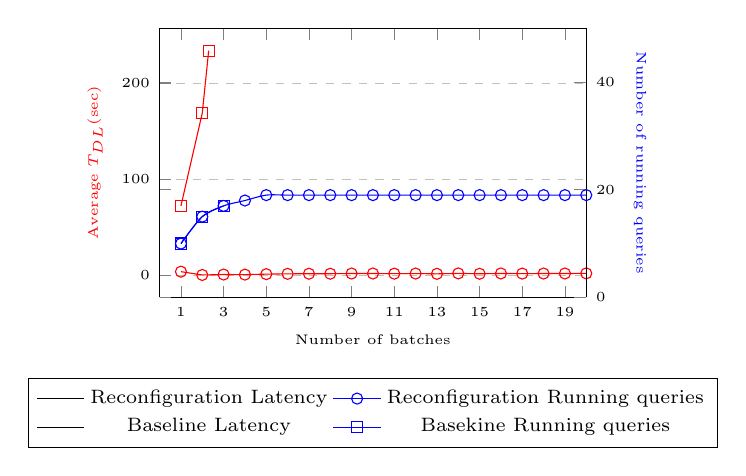
\begin{tikzpicture}
        \begin{axis}
            [
            axis y line*=left,
            ylabel style={align=center},
            xlabel style={align=center},
            xmin=0, xmax=20,
            xtick={1, 3, 5, 7, 9, 11, 13, 15, 17, 19},
            legend style={at={(0.5,-0.3)},anchor=north},
            ymajorgrids=true,
            grid style=dashed,
            axis y line*=left,
            xlabel={Number of batches},
            ylabel near ticks,
            width=7cm, height=5cm,
            label style={font=\tiny},
            legend columns=2,transpose legend,
            legend style={font=\fontsize{7}{5}\selectfont},
            ticklabel style = {font=\tiny},
            ylabel={\textcolor{red}{Average $T_{DL}$} \\\textcolor{red}{(sec)}}
            ]
            \addplot[
                color=red,
                mark=o,
            ]
            coordinates {
                (1, 3.7240590848)(2, 0.2744929792)(3, 0.7373279232)(4, 0.6528070912)(5, 1.1381799936)(6, 1.4606810112)(7, 1.5657679872)(8, 1.582769024)(9, 1.7986730752)(10, 1.8083209984)(11, 1.6307270144)(12, 1.75376)(13, 1.4564809984)(14, 1.9055259904)(15, 1.5279560448)(16, 1.8562350336)(17, 1.6939140352)(18, 1.7854290176)(19, 1.8031670272)(20, 1.942460032)
            };
            \addplot+[
            color=red,
            mark=square,
            ]
            coordinates {(1, 72.25)(2, 169.04)(2.3, 233.99)};
            \legend{Reconfiguration, Baseline}
        \end{axis}
        \begin{axis}
            [
            axis x line=none,
            xmin=0, xmax=20,
            ymin=0, ymax=50,
            legend style={at={(0.5,-0.3)},anchor=north},
            ylabel near ticks, yticklabel pos=right,
            ylabel={\textcolor{blue}{Number of running queries}},
            width=7cm, height=5cm,
            label style={font=\tiny},
            legend columns=2,transpose legend,
            legend style={font=\fontsize{7}{5}\selectfont},
            ticklabel style = {font=\tiny},
            y label style={align=center, rotate=180}
            ]
            \addlegendimage{/pgfplots/refstyle=plot:fs_10_re}\addlegendentry{Reconfiguration Latency}
            \addlegendimage{/pgfplots/refstyle=plot:fs_10_bas}\addlegendentry{Baseline Latency}
            \addlegendentry{Reconfiguration Running queries}
            \addlegendentry{Basekine Running queries}

            \addplot[blue,smooth,mark=o,domain=1:20]
            coordinates{
                (1, 10)(2, 15)(3, 17)(4, 18)(5, 19)(6, 19)(7, 19)(8, 19)(9, 19)(10, 19)(11, 19)(12, 19)(13, 19)(14, 19)(15, 19)(16, 19)(17, 19)(18, 19)(19, 19)(20, 19)
            };
            \addplot+[blue,smooth,mark=square,domain=1:20]
            coordinates{
                (1,10)(2, 15)(3, 17)
            };
        \end{axis}

    \end{tikzpicture}
    \caption{{Average $T_{DL}$} for flat topology with fluctuating workloads of 10 QPS}\label{fig:figure2}
\end{figure}

% =================================Hier======Fluctuating======10QPS===============================================================

\begin{figure}
    \centering
    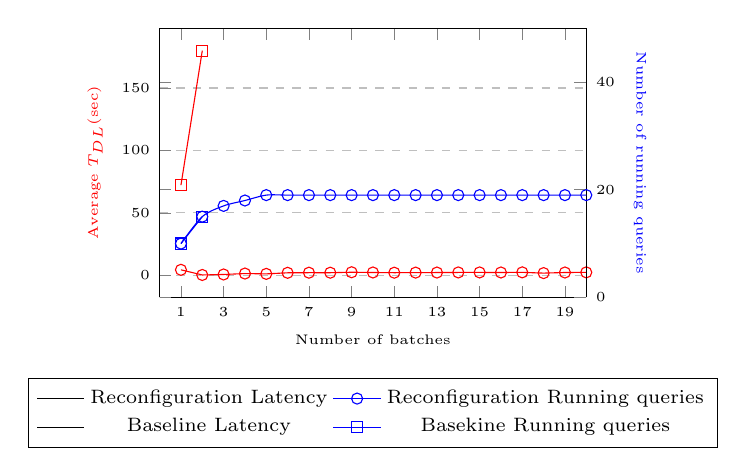
\begin{tikzpicture}
        \begin{axis}
            [
            axis y line*=left,
            ylabel style={align=center},
            xlabel style={align=center},
            xmin=0, xmax=20,
            xtick={1, 3, 5, 7, 9, 11, 13, 15, 17, 19},
            legend style={at={(0.5,-0.3)},anchor=north},
            ymajorgrids=true,
            grid style=dashed,
            axis y line*=left,
            xlabel={Number of batches},
            ylabel near ticks,
            width=7cm, height=5cm,
            label style={font=\tiny},
            legend columns=2,transpose legend,
            legend style={font=\fontsize{7}{5}\selectfont},
            ticklabel style = {font=\tiny},
            ylabel={\textcolor{red}{Average $T_{DL}$} \\\textcolor{red}{(sec)}}
            ]
            \addplot[
                color=red,
                mark=o,
            ]
            coordinates {
                (1, 4.468684928)(2, 0.3455230208)(3, 0.7413630208)(4, 1.4830230528)(5, 1.2236339968)(6, 2.0810490112)(7, 2.1697630208)(8, 2.1604089856)(9, 2.5264549888)(10, 2.3305490688)(11, 2.161709056)(12, 2.2311940608)(13, 2.2874909952)(14, 2.3689730048)(15, 2.3838960128)(16, 2.3274569216)(17, 2.4359419904)(18, 1.8413629696)(19, 2.3245420032)(20, 2.4282739712)
            };
            \addplot+[
            color=red,
            mark=square,
            ]
            coordinates {(1, 72.25)(2, 179.87)};
        \end{axis}
        \begin{axis}
            [
            axis x line=none,
            xmin=0, xmax=20,
            ymin=0, ymax=50,
            legend style={at={(0.5,-0.3)},anchor=north},
            ylabel near ticks, yticklabel pos=right,
            ylabel={\textcolor{blue}{Number of running queries}},
            width=7cm, height=5cm,
            label style={font=\tiny},
            legend columns=2,transpose legend,
            legend style={font=\fontsize{7}{5}\selectfont},
            ticklabel style = {font=\tiny},
            y label style={align=center, rotate=180}
            ]
            \addlegendimage{/pgfplots/refstyle=plot:fs_10_re}\addlegendentry{Reconfiguration Latency}
            \addlegendimage{/pgfplots/refstyle=plot:fs_10_bas}\addlegendentry{Baseline Latency}
            \addlegendentry{Reconfiguration Running queries}
            \addlegendentry{Basekine Running queries}

            \addplot[blue,smooth,mark=o,domain=1:20]
            coordinates {
                (1, 10)(2, 15)(3, 17)(4, 18)(5, 19)(6, 19)(7, 19)(8, 19)(9, 19)(10, 19)(11, 19)(12, 19)(13, 19)(14, 19)(15, 19)(16, 19)(17, 19)(18, 19)(19, 19)(20, 19)
            };
            \addplot+[blue,smooth,mark=square,domain=1:20]
            coordinates{
                (1,10)(2, 15)
            };
        \end{axis}

    \end{tikzpicture}
    \caption{{Average $T_{DL}$} for hierarchical topology with fluctuating workloads of 10 QPS}\label{fig:figure}
\end{figure}

% =================================================================================================================================20QPS===================================================================================================================================

% =======================FLAT======STABLE======20QPS===================================================================
\begin{figure}
    \centering
    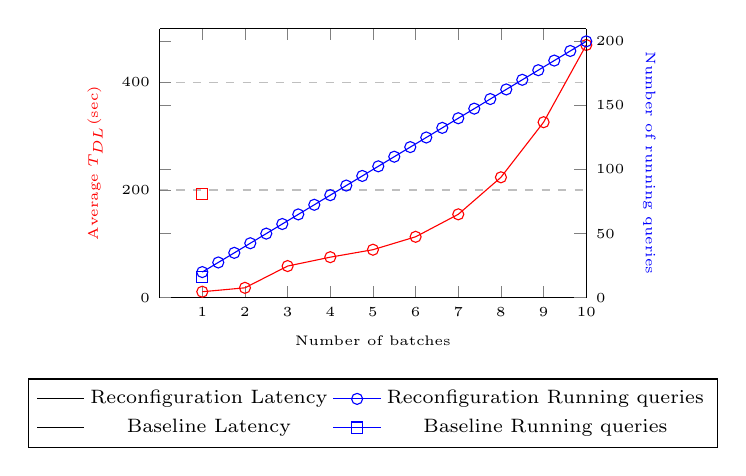
\begin{tikzpicture}

        \begin{axis}
            [
            axis y line*=left,
            ylabel style={align=left},
            xlabel style={align=center},
            xmin=0, xmax=10,
            xtick={1, 2, ..., 10},
            legend style={at={(0.5,-0.3)},anchor=north},
            ymajorgrids=true,
            grid style=dashed,
            axis y line*=left,
            ymin=0, ymax=500,
            xlabel={Number of batches},
            ylabel near ticks,
            width=7cm, height=5cm,
            label style={font=\tiny},
            legend columns=2,transpose legend,
            legend style={font=\fontsize{7}{5}\selectfont},
            ticklabel style = {font=\tiny},
            ylabel={\textcolor{red}{Average $T_{DL}$} \\\textcolor{red}{(sec)}}
            ]
            \addplot[
                color=red,
                mark=o,
            ]
            coordinates {
                (1, 11.1183854976)(2, 18.3507700096)(3, 58.785790016)(4, 75.286228992)(5, 89.157047488)(6, 113.1148860032)(7, 154.8978019968)(8, 223.6556529664)(9, 325.9963990144)(10, 469.4757604992)
            };
            \addplot+[
            color=red,
            mark=square,
            ]
            coordinates {(1, 192.63)};
        \end{axis}
        \begin{axis}
            [
            axis x line=none,
            ymin=0, ymax=210,
            xmin=0, xmax=10,
            xtick={1, 2, ..., 10},
            ylabel near ticks, yticklabel pos=right,
            ylabel style={align=left},
            ylabel={\textcolor{blue}{Number of running queries}},
            legend style={at={(0.5,-0.3)},anchor=north},
            width=7cm, height=5cm,
            label style={font=\tiny},
            legend columns=2,transpose legend,
            legend style={font=\fontsize{7}{5}\selectfont},
            ticklabel style = {font=\tiny},
            y label style={align=center, rotate=180}
            ]
            \addlegendimage{/pgfplots/refstyle=plot:fs_10_re}\addlegendentry{Reconfiguration Latency}
            \addlegendimage{/pgfplots/refstyle=plot:fs_10_bas}\addlegendentry{Baseline Latency}
            \addlegendentry{Reconfiguration Running queries}
            \addlegendentry{Baseline Running queries}

            \addplot[blue,smooth,mark=o,domain=1:10]{20*x};
            \addplot[blue,smooth,mark=square]
            coordinates {(1, 16)};
        \end{axis}

    \end{tikzpicture}
    \caption{{Average $T_{DL}$} for flat topology with stable workloads of 20 QPS}
    \label{plot:fs_20_bas}
\end{figure}

% % =======================Hier======STABLE=====20QPS====================================================================

\begin{figure}
    \centering
    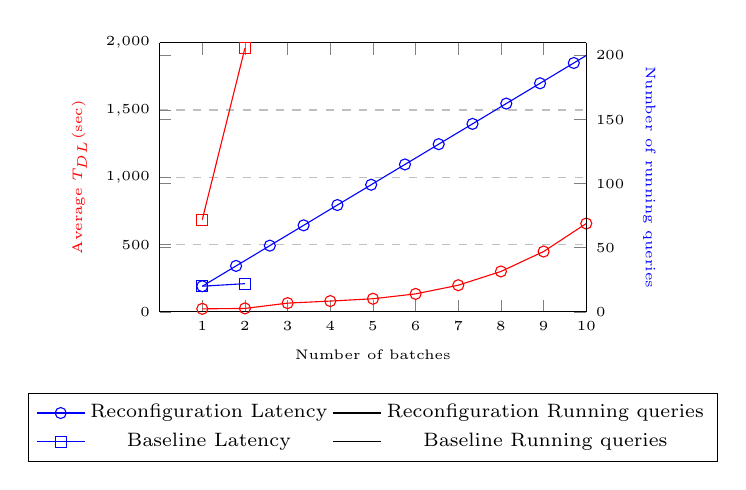
\begin{tikzpicture}
        \begin{axis}
            [
            axis y line*=left,
            ylabel style={align=left},
            xlabel style={align=center},
            xmin=0, xmax=10,
            xtick={1, 2, ..., 10},
            legend style={at={(0.5,-0.3)},anchor=north},
            ymajorgrids=true,
            grid style=dashed,
            axis y line*=left,
            ymin=0, ymax=2000,
            xlabel={Number of batches},
            ylabel near ticks,
            width=7cm, height=5cm,
            label style={font=\tiny},
            legend columns=2,transpose legend,
            legend style={font=\fontsize{7}{5}\selectfont},
            ticklabel style = {font=\tiny},
            ylabel={\textcolor{red}{Average $T_{DL}$} \\\textcolor{red}{(sec)}}
            ]
            \addplot[
                color=red,
                mark=o,
            ]
            coordinates {
                (1, 22.3873939968)(2, 25.522883008)(3, 64.9566164736)(4, 80.16785152)(5, 97.3465419776)(6, 133.5023150208)(7, 198.0004379904)(8, 300.2117550336)(9, 448.3410655104)(10, 656.3973239808)
            };
            \addplot+[
            color=red,
            mark=square,
            ]
            coordinates {(1, 685.14)(2, 1959.95)};
        \end{axis}
        \begin{axis}
            [
            axis x line=none,
            ymin=0, ymax=210,
            xmin=0, xmax=10,
            xtick={1, 2, ..., 10},
            ylabel near ticks, yticklabel pos=right,
            legend style={at={(0.5,-0.3)},anchor=north},
            width=7cm, height=5cm,
            label style={font=\tiny},
            legend columns=2,transpose legend,
            legend style={font=\fontsize{7}{5}\selectfont},
            ticklabel style = {font=\tiny},
            ylabel={\textcolor{blue}{Number of running queries}},
            y label style={align=center, rotate=180}
            ]
            \addplot[blue,smooth,mark=o,domain=1:20]{20*x};
            \addplot[blue,smooth,mark=square]
            coordinates {(1, 20)(2, 22)};
            \addlegendimage{/pgfplots/refstyle=plot:fs_10_re}\addlegendentry{Reconfiguration Latency}
            \addlegendimage{/pgfplots/refstyle=plot:fs_10_bas}\addlegendentry{Baseline Latency}
            \addlegendentry{Reconfiguration Running queries}
            \addlegendentry{Baseline Running queries}
        \end{axis}
    \end{tikzpicture}
    \caption{{Average $T_{DL}$} for hierarchical topology with stable workloads of 20 QPS}
    \label{fig:tdt_hier_stable_20}
\end{figure}


% % =================================FLAT======Fluctuating====20QPS===================================================

\begin{figure}
    \centering
    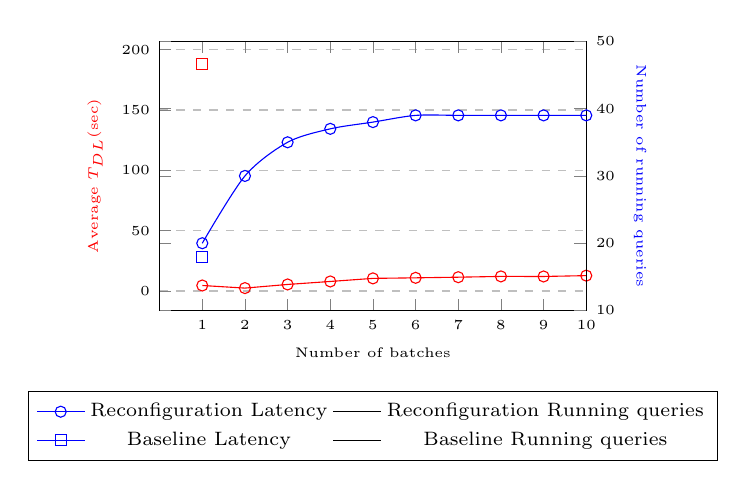
\begin{tikzpicture}
        \begin{axis}
            [
            axis y line*=left,
            ylabel style={align=left},
            xlabel style={align=center},
            xmin=0, xmax=10,
            xtick={1, 2, ..., 10},
            legend style={at={(0.5,-0.3)},anchor=north},
            ymajorgrids=true,
            grid style=dashed,
            axis y line*=left,
            xlabel={Number of batches},
            ylabel near ticks,
            width=7cm, height=5cm,
            label style={font=\tiny},
            legend columns=2,transpose legend,
            legend style={font=\fontsize{7}{5}\selectfont},
            ticklabel style = {font=\tiny},
            ylabel={\textcolor{red}{Average $T_{DL}$} \\\textcolor{red}{(sec)}}
            ]
            \addplot[
                color=red,
                mark=o,
            ]
            coordinates {
                (1, 4.5889169792)(2, 2.4340605056)(3, 5.4577880192)(4, 7.9318400512)(5, 10.485785984)(6, 10.946873472)(7, 11.469816)(8, 12.118257984)(9, 12.066668992)(10, 12.7684120064)
            };
            \addplot+[
            color=red,
            mark=square,
            ]
            coordinates {(1, 188.34)};
        \end{axis}

        \begin{axis}
            [
            axis x line=none,
            ymin=10, ymax=50,
            xmin=0, xmax=10,
            xtick={1, 2, ..., 10},
            ylabel near ticks, yticklabel pos=right,
            legend style={at={(0.5,-0.3)},anchor=north},
            width=7cm, height=5cm,
            label style={font=\tiny},
            legend columns=2,transpose legend,
            legend style={font=\fontsize{7}{5}\selectfont},
            ticklabel style = {font=\tiny},
            ylabel={\textcolor{blue}{Number of running queries}},
            y label style={align=center, rotate=180}
            ]
            \addplot[blue,smooth,mark=o]
            coordinates {(1, 20)(2, 30)(3, 35)(4, 37)(5, 38)(6, 39)(7, 39)(8, 39)(9, 39)(10, 39)};
            \addplot[blue,smooth,mark=square]
            coordinates {(1, 18)};
            \addlegendimage{/pgfplots/refstyle=plot:fs_10_re}\addlegendentry{Reconfiguration Latency}
            \addlegendimage{/pgfplots/refstyle=plot:fs_10_bas}\addlegendentry{Baseline Latency}
            \addlegendentry{Reconfiguration Running queries}
            \addlegendentry{Baseline Running queries}
        \end{axis}
    \end{tikzpicture}
    \caption{{Average $T_{DL}$} for flat topology with fluctuating workloads of 20 QPS}
    \label{fig:tdt_stable_fluc_20}
\end{figure}

% % ==============================Hier======Fluctuating====20QPS==================================================================

\begin{figure}
    \centering
    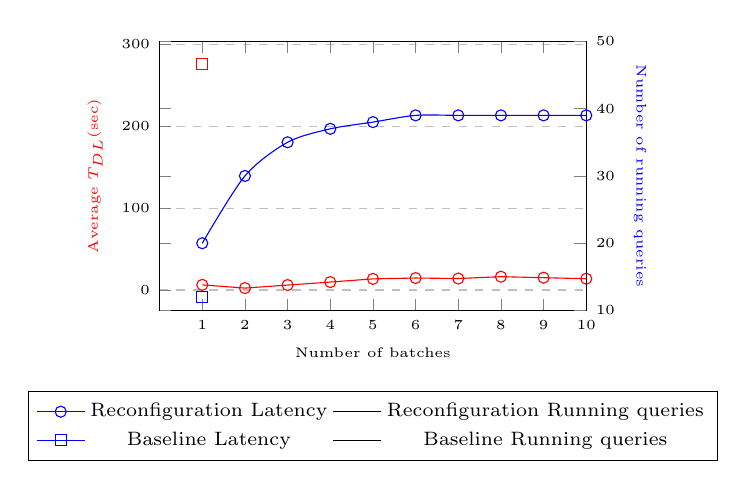
\begin{tikzpicture}
        \begin{axis}
            [
            axis y line*=left,
            ylabel style={align=left},
            xlabel style={align=center},
            xmin=0, xmax=10,
            xtick={1, 2, ..., 10},
            legend style={at={(0.5,-0.3)},anchor=north},
            ymajorgrids=true,
            grid style=dashed,
            axis y line*=left,
            xlabel={Number of batches},
            ylabel near ticks,
            width=7cm, height=5cm,
            label style={font=\tiny},
            legend columns=2,transpose legend,
            legend style={font=\fontsize{7}{5}\selectfont},
            ticklabel style = {font=\tiny},
            ylabel={\textcolor{red}{Average $T_{DL}$} \\\textcolor{red}{(sec)}}
            ]
            \addplot[
                color=red,
                mark=o,
            ]
            coordinates {
                (1, 6.2433320192)(2, 2.2886989568)(3, 5.97854848)(4, 9.6494655104)(5, 13.5501744896)(6, 14.5781735168)(7, 13.9808100096)(8, 16.2264104576)(9, 14.9915455232)(10, 13.7347549952)
            };
            \addplot+[
            color=red,
            mark=square,
            ]
            coordinates {(1, 276.13)};
        \end{axis}

        \begin{axis}
            [
            axis x line=none,
            ymin=10, ymax=50,
            xmin=0, xmax=10,
            xtick={1, 2, ..., 10},
            ylabel near ticks, yticklabel pos=right,
            legend style={at={(0.5,-0.3)},anchor=north},
            width=7cm, height=5cm,
            label style={font=\tiny},
            legend columns=2,transpose legend,
            legend style={font=\fontsize{7}{5}\selectfont},
            ticklabel style = {font=\tiny},
            ylabel={\textcolor{blue}{Number of running queries}},
            y label style={align=center, rotate=180}
            ]
            \addplot[blue,smooth,mark=o]
            coordinates {(1, 20)(2, 30)(3, 35)(4, 37)(5, 38)(6, 39)(7, 39)(8, 39)(9, 39)(10, 39)};
            \addplot[blue,smooth,mark=square]
            coordinates {(1, 12)};
            \addlegendimage{/pgfplots/refstyle=plot:fs_10_re}\addlegendentry{Reconfiguration Latency}
            \addlegendimage{/pgfplots/refstyle=plot:fs_10_bas}\addlegendentry{Baseline Latency}
            \addlegendentry{Reconfiguration Running queries}
            \addlegendentry{Baseline Running queries}
        \end{axis}
    \end{tikzpicture}
    \caption{{Average $T_{DL}$} for hierarchical topology with fluctuating workloads of 20 QPS}
    \label{fig:tdt_hier_fluc_20}
\end{figure}